\section*{Tutorial Relasi Antar Table}
\begin{enumerate}
	
	\item Sebelum membuat relasi antar tabel kita di wajibkan menghapus primary key pada setiap tabel, primary key yang dimaksud adalah "ID".  
	
	\item Klik Data Workshop dan cari tabel yang akan kita hapus primary key nya, disini saya akan menghapus primary key pada tabel mhs, tabel dosen, tabel matul, tabel jadwal, dan tabel nilai. Perintah yang di klik untuk menghapus primary key adalah "Drop Column", lalu isikan column yang akan kita hapus pada form "Remove column" lalu klik next    
	\begin{figure} [!htbp]
	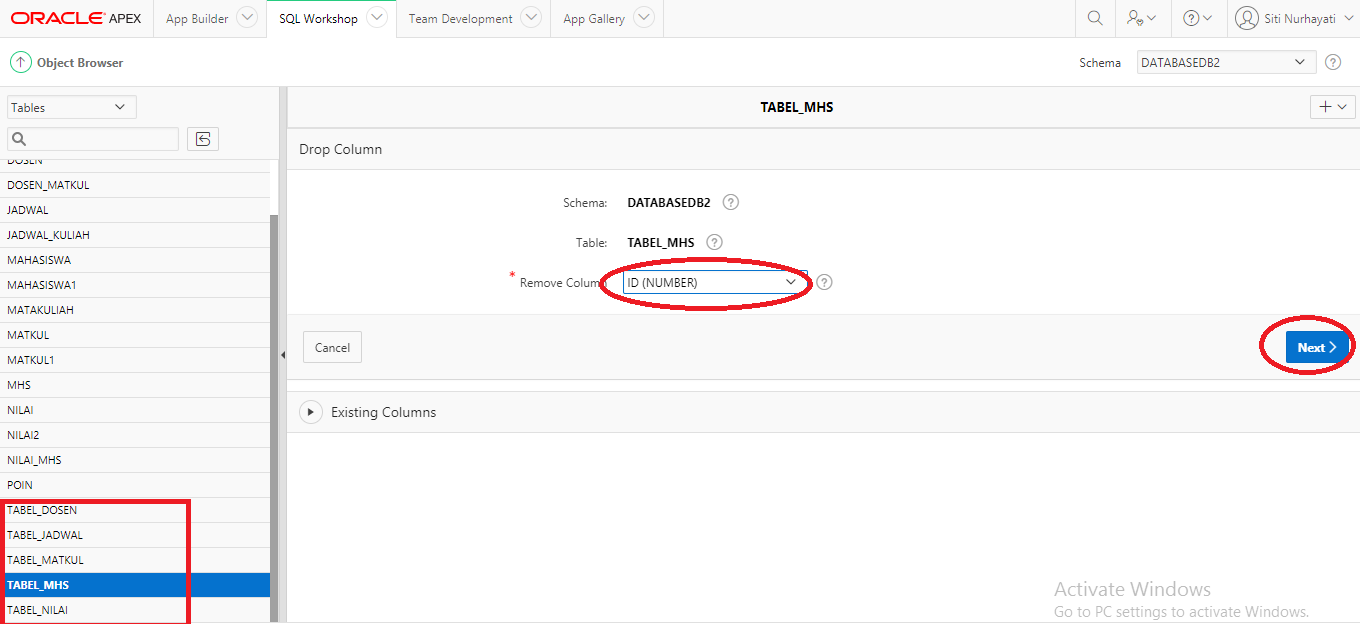
\includegraphics[scale=0.2]{Apex/18a.png}
	\centering
	\end{figure}
	
	\item Setelah primary key "ID" sudah dihapus maka buatlah primary key baru menggunakan Query seperti dibawah ini, dilakukan juga di tabel dosen, tabel jadwal, tabel matakuliah, dan tabel nilai lalu klik "run"
	\begin{figure} [!htbp]
	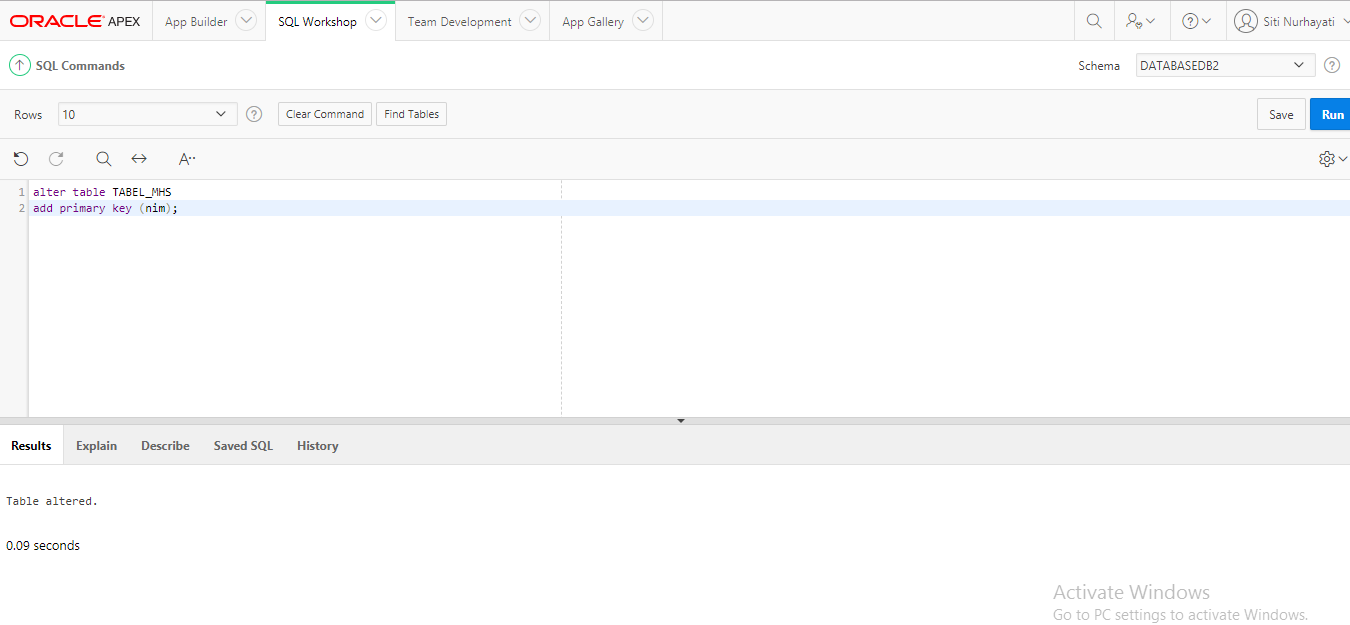
\includegraphics[scale=0.2]{Apex/19.png}
	\centering
	\end{figure}
	
	\item Untuk menambahkan foreign key menggunakan query seperti dibawah ini lalu klik run 
	\begin{figure} [!htbp]
	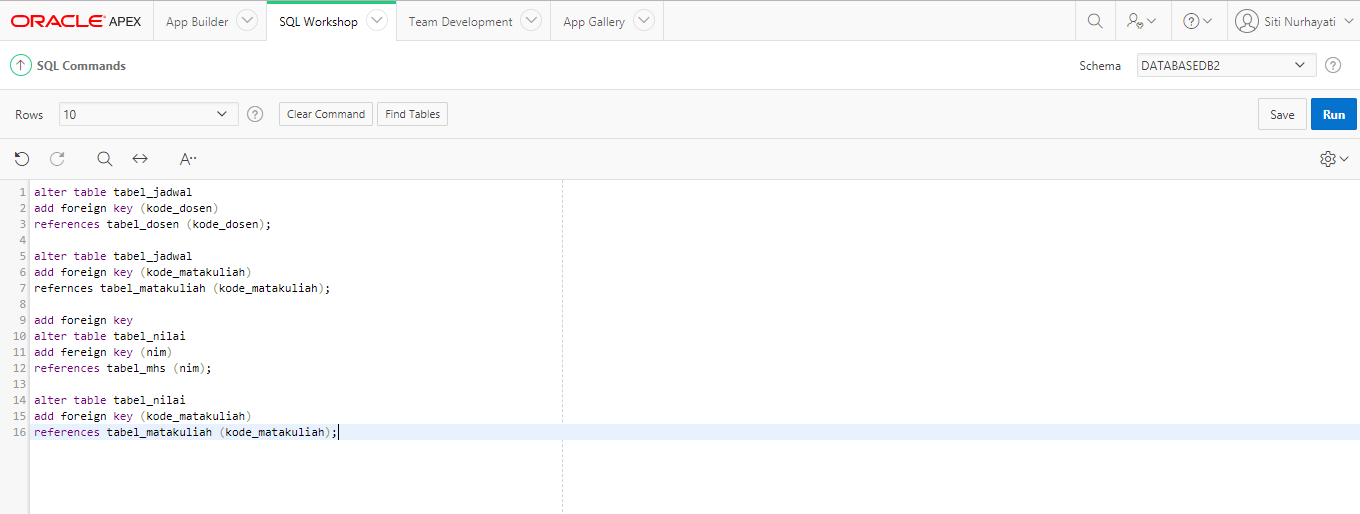
\includegraphics[scale=0.2]{Apex/a.png}
	\centering
	\end{figure}

\end{enumerate}
